%%%%%%%%%%%%%%%%%%%%%%%%%%%%%%%%%%%%%%%%%%%%%%%%%%%%%%%%%%%%
%%%%%%%%%%%%%%%%%%%%%%%%%%%%%%%%%%%%%%%%%%%%%%%%%%%%%%%%%%%%
%%%%%%%%%%%%%%%%%%%%%%%%%%%%%%%%%%%%%%%%%%%%%%%%%%%%%%%%%%%%
\section{Introduction}
%%%%%%%%%%%%%%%%%%%%%%%%%%%%%%%%%%%%%%%%%%%%%%%%%%%%%%%%%%%%
%%%%%%%%%%%%%%%%%%%%%%%%%%%%%%%%%%%%%%%%%%%%%%%%%%%%%%%%%%%%
%%%%%%%%%%%%%%%%%%%%%%%%%%%%%%%%%%%%%%%%%%%%%%%%%%%%%%%%%%%%

\subsection{PDELab Aims and Features}

\begin{frame}
\frametitle<presentation>{DUNE PDELab Features}
\begin{itemize}
\item Rapid prototyping: Substantially reduce time to implement
discretizations and solvers for systems of PDEs based on DUNE.
\item Simple things should be simple --- suitable for teaching.
\item Discrete function spaces spaces:
\begin{itemize}
\item Conforming and non-conforming,
\item hp-refinement,
\item general approach to constraints,
\item generic generation of product spaces for systems.
\end{itemize} 
\item Operators based on weighted residual formulation:
\begin{itemize}
\item Linear and nonlinear,
\item stationary and transient,
\item FE and FV schemes requiring at most face-neighbors.
\end{itemize} 
\item Exchangeable linear algebra backend. 
\item User only involved with ``local'' view on (reference) element.
\end{itemize}
\end{frame}

\begin{frame}
\frametitle<presentation>{DUNE Module Architecture}
Major DUNE modules are:
\begin{center}
\mode<presentation>{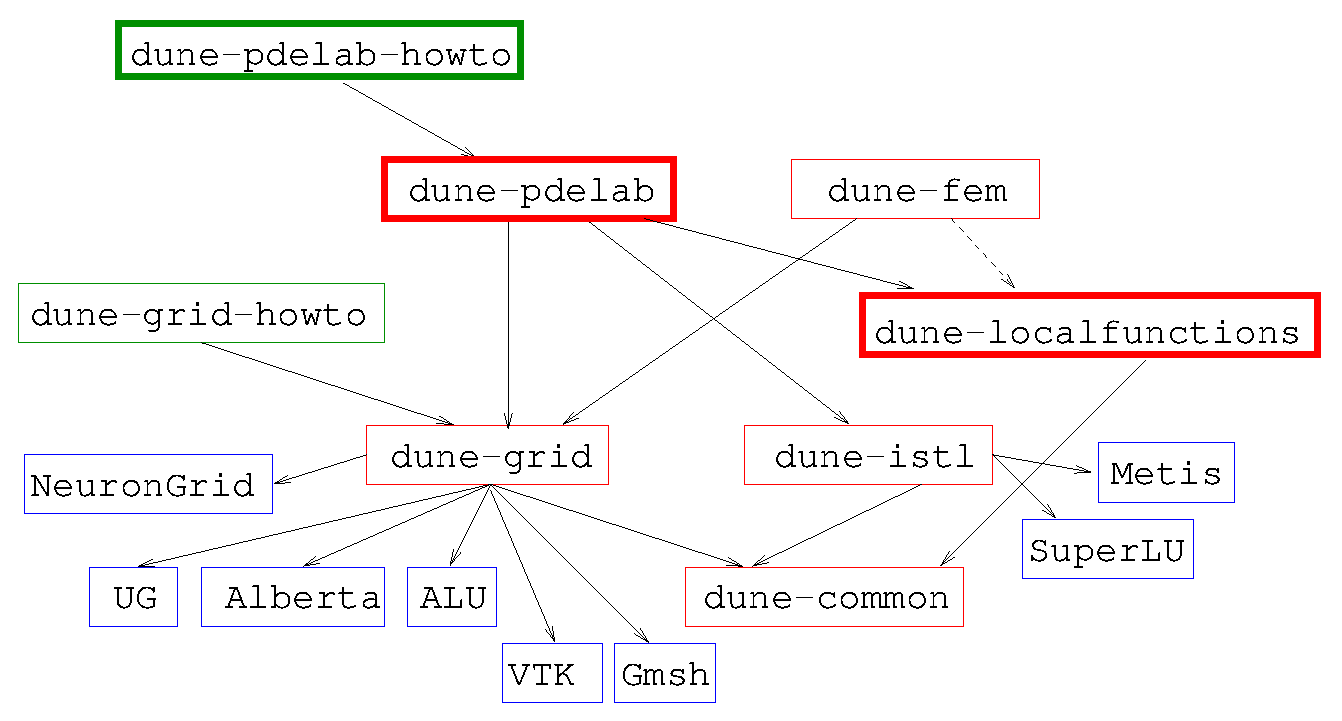
\includegraphics[width=1.0\textwidth]{./EPS/modules}}
\mode<article>{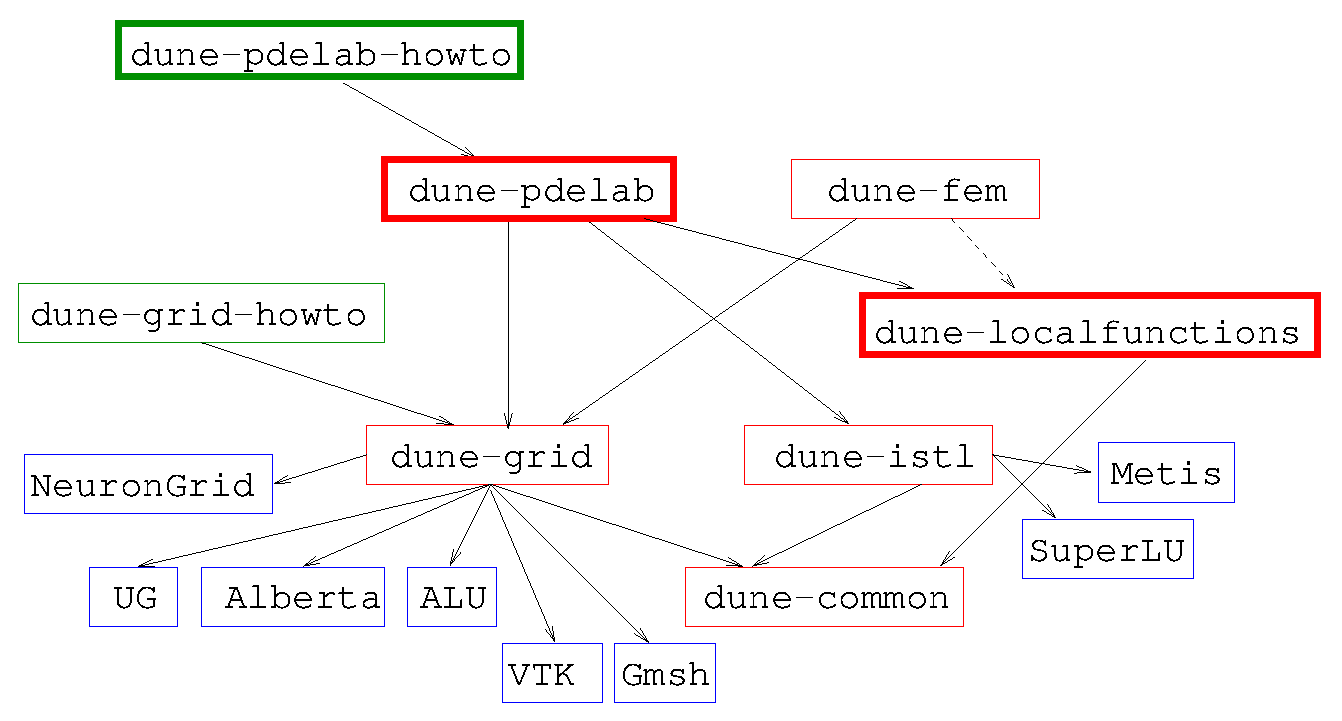
\includegraphics[width=0.7\textwidth]{./EPS/modules}}
\end{center}
\end{frame}

\begin{frame}
\frametitle<presentation>{Required Modules}
To work through the examples the following DUNE modules are required: 
\begin{itemize}
\item \lstinline{dune-common},
\item \lstinline{dune-grid},
\item \lstinline{dune-istl},
\item \lstinline{dune-localfunctions},
\item \lstinline{dune-pdelab},
\item \lstinline{dune-pdelab-howto},
\end{itemize}

In addition, at least one of the grid managers UG, ALU or Alberta is
required to do the examples on simplex grids. 
\end{frame}



\subsection{How to Read this Manual}

Section 2 introduces the \textit{weighted residual formulation} which
is the abstract formulation of PDE problems in PDELab. You should at
least get some idea about it on your first reading.

Section 3 presents the theory behind grid function
spaces including the constuction of subspaces due to general
constraints. An understanding of this is necessary if you want to
implement new function spaces or constraints.

Section 4 provides a step by step introduction to the implementation
of grid function spaces. Working through these examples will enable
you to use existing function spaces and implement new ones.

Section 5 contains the theory behind the solution of the algebraic
systems arising from the constrained weigthed residual formulation.

Section 6 then shows how a discretization scheme is implemented using
the grid function spaces. A simple conforming discretization of the
Laplacian is worked through in detail and the set-up of solvers
using \lstinline{dune-istl} is explained.

Section 7 contains a list of the problems implemented in
the \lstinline{examples} directory.

\cleardoublepage
